\documentclass[a4paper, 12pt]{article}

%% Language and font encodings
\usepackage[english]{babel}
\usepackage[utf8x]{inputenc}
\usepackage[T1]{fontenc}
\usepackage{float}

%% Sets page size and margins
\usepackage[a4paper,top=3cm,bottom=2cm,left=3cm,right=3cm,marginparwidth=1.75cm]{geometry}

%% Imports pictures
\usepackage{graphicx}
\usepackage{subcaption}
\graphicspath{{./Pictures/}}

%% Sets line and paragraph spacing
%\setlength{\parindent}{4em}
\setlength{\parskip}{1em}
\renewcommand{\baselinestretch}{1.5}

%% Useful packages
\usepackage{amsmath}
\usepackage{graphicx}
\usepackage[colorinlistoftodos]{todonotes}
\usepackage[colorlinks=true, allcolors=blue]{hyperref}
\usepackage{pgfgantt} % Used for Gantt Chart

%% Title
\title{Final Report}
\author{Ahmad AlKhoory, Zihao Zhao, Nien-Tsu Chou, Xiang Li,\\Mohammad Omdah, and Shiyu Zhang}
\date{March 27, 2018}

\begin{document}
\maketitle


%% Introduction
\section{Introduction}
Ray tracing is a rendering technique that can produce incredibly realistic lighting effects. Essentially, an algorithm can trace the path of light, and then simulate the way that the light interacts with the virtual objects it ultimately hits in the computer-generated world \cite{Ray tracing}. It is widely used in movie industry, architectural design and game engines. The work has been done is to build an application for the algorithm which enables users to create their own figures by configuring all parameters about the scene and objects. After doing some research about the algorithm, the load has been divided into three parts: Shape Design, Ray Tracing Implementation (the back-end) and Graphical User Interface (the front-end).

Whenever a server is open in a local area network (LAN), users can access to the application by visiting corresponding IP with certain port using their laptops, desktops or smart phones. Since the application has been deployed to the cloud, whoever has Internet access can use the application and generate the ray tracing figure.

While using the application, a JSON file is generated by the front-end after all the parameters about the scene and objects (object type, transparency, color, camera position, light source coordinates, etc) are successfully collected.

Eventually, the Json file can be read by the back-end which defines the the shapes from mathematical calculation of Geometry with all the features of scene and objects have been input, after that the rendering of the image will be presented.

After two months of researching, programming and testing, the team has accomplished the requirements of the project. Basically, the task has been distributed between the team members in groups of two. The first group is responsible for shapes design, the second one is responsible for raytracing and integration with the front end and the last one is responsible for GUI. The team decided to use Python as programming language for ray tracer back-end and GUI. In addition to Python, HTML, JavaScript and JQuery are also used in GUI. 

This report demonstrates how the project has been completed in terms of requirements, which includes how each part has been designed, implemented, and tested. Moreover, the report highlighted how the teamwork has been processed, conflicts been handled, and evaluation and peer assessment been agreed on.


%% Requirements and Design
\section{Requirements and Design}

\subsection{Shapes Design}
Shape design group was caring of mathematical and physics theory to design shapes to the code. The formulas of line, point in the space, light source ,vectors algebra and matrices were followed to achieve the design, then each shape has it own calculation.

\subsubsection{Vector algebra}
The vector arithmetic equations are important to understand the design. A 3D vector can be  represented as: $P=\left[\begin{matrix}x\\y\\z\\\end{matrix}\right]$, the length of the vector is equal to the magnitude: $|P|=\sqrt{x^2+y^2+z^2}$, consequently if we have two vectors: The dot product A = (xa, ya, za) and B = (xb, yb, zb) is: $A\cdot B = xa xb + ya yb + za zb$, the dot product is a scalar value equal to: $A.B=\left|A\right||B|\cos{\theta}$, where $\theta$ is the angle between the two vectors.

Note that if A= B this means that: $P.P={|P|}^2$. Also note that the dot product between two mutually perpendicular vectors is always zero. However, the cross of two vectors is different because result to new vector orthogonal on both cross vectors.

The cross product of two vectors is new vector cab be represented as: $$A\times B=\left[\begin{matrix}yazb - zayb \\ zaxb - xazb \\ xayb - yaxb \\\end{matrix}\right]$$, the orthogonal vector direction determined by using right hand side rule by putting index finger to vector A and middle finger to vector B, the thumb finger showing the direction of the new vector \cite{Ray tracing primitives}.

Another concept should be learned is the concept of matrix multiplication, if we have a Vector point Pv with 3 values (x,y,z) this can be represented in matrix 1x3. The  multiplication of this matrix with any matrix should be with 3 rows. It can be generalized as  Pv = mxp multiply by Pn = pxn, the results transfer point Pt = mxn. To demonstrate this, consider Pv = 1x3 and Pn = 3x3, the result is Pt = 1x3.

$$Pt = \begin{matrix} (x&y&z)*\left[\begin{matrix}P00&P01&P02\\P10&P11&P12\\P20&P21&P22\\\end{matrix}\right]\end{matrix}$$

This results to:\\
Pt.x = P.x * P00 + P.y * P10 + P.z * P20 \\
Pt.y = P.x * P01 + P.y * P11 + P.z * P21 \\
Pt.z = P.x * P02 + P.y * P12 + P.z * P22 \cite{Learn Computer Graphics From Scratch}

\subsubsection{Ray Equation}
A ray can be identified by an origin or eye point $E(x_E,y_E,z_E)$ and an offset vector, $D=(x_D,y_D,z_D)$ . The ray equation can be written: $P(t)=E+tD, t\geq 0$.
Actually, this can be represented in three equations: Where $ t \geq 0: x(t)=xE+txD, y(t)=yE+tyD, z(t)=zE+tzD$.

If a ray-object intersection point was found, this means the eye are looking for the intersection point with the lowest non-negative value of (t). The ray-tracing algorithm takes an image made of pixels. For each pixel in the image, it looks a primary ray into the scene. The direction of that primary ray is rendered by tracing a line from the eye to the center of that pixel. Once the primary ray's direction set, each object of the scene to see if it intersects with any of them. Check Figure \ref{fig:EyetoObject}. Now, the above equations can be applied to many objects and each of them have different calculation according to the shape.

\begin{figure}[h] 
\centering
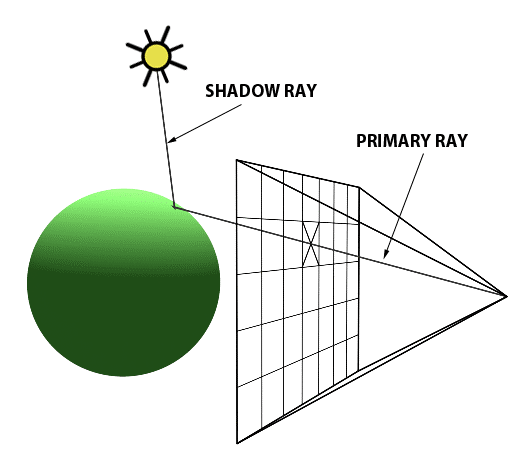
\includegraphics[scale=0.3]{ShD_light_source.png}
  \caption{Eye to Object}
   \label{fig:EyetoObject}
\end{figure}

To deal easily with the various primitive objects in standard 3D coordinate systems: rectangular $(x,y,z)$, spherical polar $(r, \Theta, \phi)$, and cylindrical polar $(r, \Theta, z)$. To convert from one to another the following formula can be used:

Spherical polar to rectangular: $x=r\cos{\varphi}\cos{\theta}, y=r\cos{\varphi}\sin{\theta}, z=r\sin{\varphi}$

Cylindrical polar to rectangular: $x=r\cos{\theta}, y=r\sin{\theta}, z=z$


Rectangular to spherical polar: $r=\sqrt{x^2+y^2+z^2}, \theta=\tan^{-1}{\frac{y}{x}}, \varphi=\tan^{-1}{(\frac{z}{\sqrt{x^2+y^2}})}$

Rectangular to cylindrical polar: $r=\sqrt{x^2+y^2}, \theta=\tan^{-1}{\frac{y}{x}}, z=z$ 
\cite{Learn Computer Graphics From Scratch}

\subsubsection{Sphere}
The unit sphere, centered at the origin, the ray tracing can be defined by position  and radius the equation is: $x^2+y^2+z^2=1$, and in spherical polar coordinates it is even simpler: $r=1$, in vector arithmetic, it becomes: $P.P=1$. To find the intersection between this sphere and an arbitrary ray, substitute the ray equation in the sphere equation, after the calculation the result is: $t=\frac{-b\pm\sqrt{b^2-4ac}}{2a}$, where: $$a=x_{D^2}+y_{D^2}+z_{D^2}, 
b={2 x_E x_D + 2 y_E y_D + 2 z_E z_D}, c=x_E^2 + y_E^2 + z_E^2 - 1 $$

t gives zero, one, or two real values for t. If there are zero real values then there is no intersection between the ray and the sphere. If there are either one or two real values then chose the smallest, non-negative value, as the intersection point. If there is no non-negative value, then the line (of which the ray is a part) does intersect the sphere, but the intersection point is not on the part of the line which constitutes the ray. In this case there is again no intersection point between the ray and the sphere \cite{Ray tracing primitives}.

\subsubsection{Cylinder}
The infinite unit cylinder aligned along the z-axis, cylinder can be be defined in ray tracing by position, height and radius. The mathematical calculation: $x^2+y^2=1$. In cylindrical polar coordinates it is just $r=1$.

After applying the ray intersect equation in cylinder equation equation will have: 
$$a=x_D^2+y_D^2, b=2 x_E x_D + 2 y_E y_D, c=x_E^2+y_E^2-1$$

Same thing has been done for cone, tetrahedron and cube to define the requirements and  do the calculation ray equations, intersection plan and position \cite{Ray tracing primitives}.

\subsection{RayTracing Design}
At the beginning of project, we decided to develop our software base on a Python sample code \cite{Very simple ray-tracing engine in (almost) pure Python} for the reason that we do not have to build from scratch. Then, we set few requirements such as adding more shapes, adjusting the reflectivity of the objects, as well as controlling the camera and light source positions which the sample code did not provide. We decided to improve performance before implementing other functionality because it will reduce the testing time in whole project process. We chose multi-processing as a main solution for this issue because it can easily improve overall performance. Each subgroup member is assigned to develop some of functionality. For example, the method of finding intersection with ray and different shapes can be developed independently, so we decided that each member work on this method with one or two shapes. For input file analyze, because it related to parameters of each shape and input represented in front end, the developer plays a role of bridge between shapes and GUI design. Also, we decided to use JSON format because it is python friendly and our team were more familiar with it.

\subsection{GUI Design}
The GUI was initially planned to be designed using a tool called Kivy, which is a new open source Python library for application development, that makes use of innovative user interfaces, such as multi-touch applications \cite{kivy}. However, after struggling with Kivy for longer than a month, with poor improvement to our targeted GUI, we decided to move to a web-based platform, particularly using Flask, which is a micro framework for Python. The web-based GUI can be separated into two parts: the HTML page design, and the Flask event response logic design.


%% Implementation
\section{Implementation}
This section is divided into three subsections, particularly Shapes Implementation, RayTracing Implementation, and GUI Implementation. Each subsection will cover the technicality of the implementation process, and how each group developed their part to the final desired product.

\subsection{Shapes Implementation}
Shape design aims to draw three-dimensional graphics through the Python language, which provides a graphical basis for subsequent ray tracing and back-end execution work. According to the graphical requirements proposed in the requirements, the shape design section will add sphere, tetrahedron, cube, cylinder, and cone to the code.

\subsubsection{Sphere}
With the demo code of the sphere, the output can be generated by changing the different input of the basic attributes like color, position, radius and intersection plane. The three numerical inputs allow users to decide from the GUI interface to construct the shape: coordinate of the sphere center and radius to decide the size and position of the sphere, RGB of color to optimize the appearance. Users can draw any number of balls they want by adding these three basic graphics attributes in turn.

Below is the sphere code, the output results as seen in Figure \ref{fig:Sphere Code} and \ref{fig:RayIntersection} and \ref{fig:SphereShape}:

\begin{figure}[h]
\centering
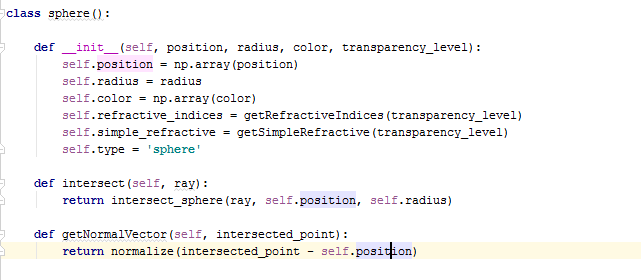
\includegraphics[scale=0.6]{ShD_Sphere_code.png}
  \caption{Sphere Code}
  \label{fig:Sphere Code}
\end{figure}

\begin{figure}[ht]  
\centering
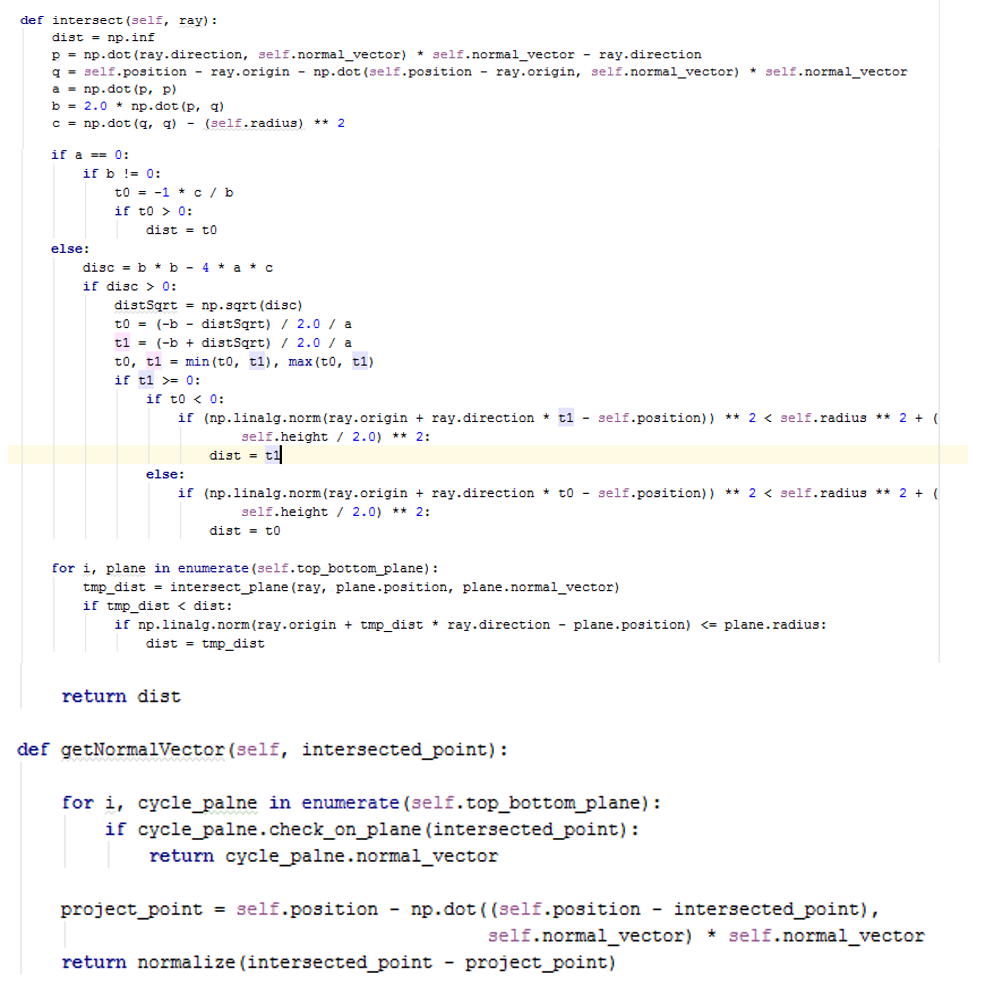
\includegraphics[scale=0.6]{ShD_ray_intersection_code.png}
    \caption{Ray Intersection Code}
    \label{fig:RayIntersection}
\end{figure}


\subsubsection{Shape Design Software testing}
In the process of code testing, once there was the following error message. It happens in the python version 2.7 because the results of the division are taken as integers. There are some of solutions as follows as we can see in Figure \ref{fig:Error}:

\begin{enumerate}
\item Make x project an integer by add int().
\item Import division module from future import division
\item Change / into //
\end{enumerate}


Some of the team was using Python version 3.6 and this version no error with division taken as integers. Also , another error message with print function with different version of Python, However , all the team has agreed to use python 2.7 and update the code according to the error of this version.

\begin{figure}[htbp]
\centering
\begin{minipage}[t]{0.38\textwidth}
\centering
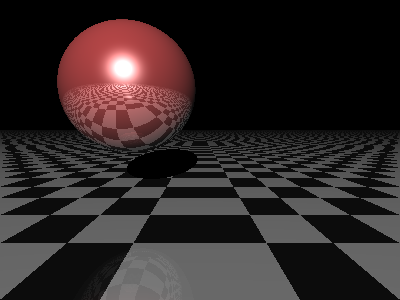
\includegraphics[width=4cm]{ShD_Sphere_Pic.png}
\caption{Sphere Shape}
\label{fig:SphereShape}
\end{minipage}
\begin{minipage}[t]{0.48\textwidth}
\centering
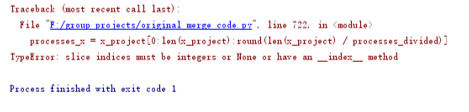
\includegraphics[width=10cm]{ShD_error_message.png}
\caption{Error Message}
\label{fig:Error}
\end{minipage}
\end{figure}


\subsubsection{Time Testing}
The time testing result to run the back-end was 1 min 20 sec. Basically, this computation because the image output pixels width and height was increased to 512 * 512. Also , it depends on machine RAM memory for higher memory less time. Below Figure \ref{fig:Timetestingpart4} is showing that.

\begin{figure}[H]
\centering
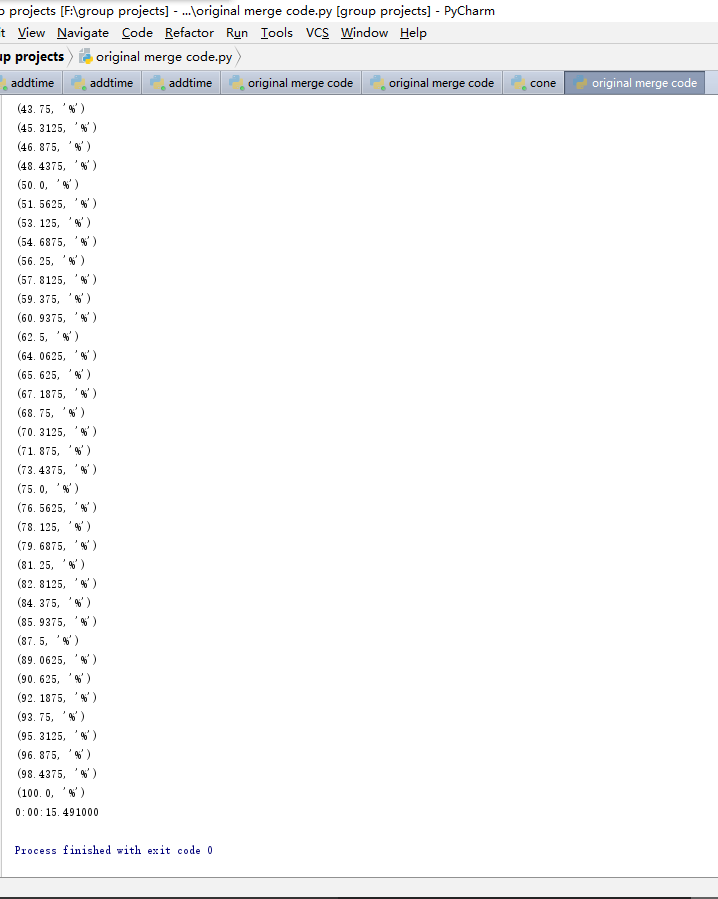
\includegraphics[scale=0.4]{ShD_Timetesting_part4.png}
  \caption{Timetesting}
     \label{fig:Timetestingpart4}
\end{figure}

\subsection{RayTracing Implementation}
RayTracing implementation aims to figure out how rays and shapes interact in a scene to contribute the colour in a raster image. Also, this part takes up most of the running time in the software. As a result, we will mention the performance issue and how we addressed in this subsection.

\subsubsection{Intersection}
When a ray intersects an object, it is necessary to find the intersection point. However, depend on the different shape, the way to find the intersection point is different as well. In this report, we will demonstrate how the intersection works on sphere and cube. The reason why we choose the sphere and cube is that first, the sphere is the simplest shape, once we figure that out, we can easily apply the method to other spherical shape. Second, we used the special technique to deal with the cube.

1. Sphere

As we mentioned before in the Shape Integration part, the sphere can be defined by position and radius. The equation for a sphere is: $$ x^2 + y^2 + z^2 = R^2$$

Where x, y and z are the coordinates of a cartesian point and R is the radius. When we want to get the distance between the ray and the sphere, we can calculate the equation by re-write the equation:(O+tD defines all points along the ray) $$|O+ tD|^2 - R^2 = 0$$

When we carry on, we can get the new equation: $$D^2t^2+ 2ODt - O^2 - R^2= 0$$ With $a = D^2$, $b = 2OD $, $c = O^2 - R^2$, we can get $\Delta= b^2 - 4ac$

\begin{itemize}

\item When $\Delta < 0$, there is no root, which means the ray doesn't intersect the object. So the return value is inf.

\item When $\Delta = 0$, there is one root: $$-\frac{b}{2a}$$ Which means $t_0 = t_1$.

\item When $\Delta > 0$, there is two roots: $$\frac{-b + \sqrt{\Delta}}{2a}\quad and\quad \frac{-b + \sqrt{\Delta}}{2a}$$ In this case, the ray intersects the sphere with two places ($t_0\, and\, t_1$). However, we only choose the closest one because that is the place where ray first intersect with object and later then the ray will not reach the further one.

The ray-sphere intersection code is as shown in Figure \ref{fig:Ray Sphere}.
\end{itemize}

\begin{figure}[htb]
\centering
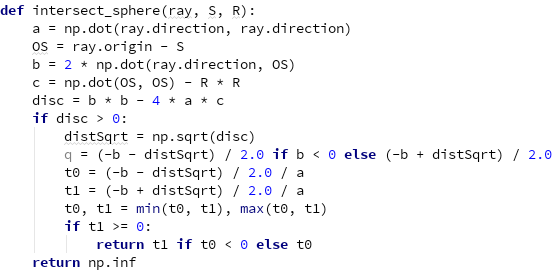
\includegraphics[scale=0.75]{ray_sphere.png}
\caption{Ray Sphere}
\label{fig:Ray Sphere}
\end{figure}  

2. Cube

Different from the sphere, the cube has eight sides, which means we can not use the old method (sphere one) to calculate the intersection place.

For this reason, we apply the new method called 'spli\_square\_to\_triangle' on the cube. In the computer graphical design, everything can be split into many triangle planes. Same on cube, we split every surface of cube into two triangles. After that, we add these triangle planes into triangleSet. Then we calculate the intersection between triangleSet and the ray.

For every triangle plane, we first judge whether the ray will intersect the infinite plane (which cover the triangle plane) or not. If not, skip this plane. If it is, then we calculate if the intersection point in the triangle plane by using method 'PointinTriangle'. By doing this iteration, we can finally know the intersection point of the ray on the cube and the distance between them.

However, the performance is not satisfied. Because for every cube, we need to do the calculation eight times, which will pull down the capability. If the ray doesn't intersect the cube, the previous calculation is totally wasted. To avoid that, we come up with a new idea which can reduce the computation.

As we all know, the cube is bounded by six equal squares and every edge of it is the same. In another words, the eight point of the cube has the same distance to its centre, which is similar to sphere (every point on its surface equidistant from its centre). Based on that definition, we first transmit the cube into sphere with $radius = \frac {\sqrt 3a}{2}$ ($a$ is the length of cube).

From now on, we only check whether the ray will intersect with sphere or not. If not, we skip this cube. If it is, then we calculate the eight triangle planes. This method save a lot of time and increase the performance.

\subsubsection{Reflection and Refraction}
When a ray intersects a surface of an object, reflection ray and refraction ray are generated. When these rays intersect another object in a scene, each ray will generate two more rays (Figure \ref{fig:Reflection and Refraction}). The recursive function reflect$\_$and$\_$refract() calculates the colour of objects which are interacted with each depth of reflective and refractive ray and determine the final RGB colour value of a pixel as seen in Figure \ref{fig:Recursion of reflection and refraction}. To generate a more realistic image, this function uses Fresnel equation \cite{Learn Computer Graphics From Scratch} to calculate how much light an object reflects and refracts instead of just always using the fixed reflectivity amount of the object. Fresnel Equation is stated below:

\[Reflective\ Amount = \frac{1}{2}((\frac{n_2\cos{\theta_1} - n_1\cos{\theta_2}}{n_2\cos;{\theta_1} + n_1\cos{\theta_2}})^2 + (\frac{n_1\cos{\theta_2} - n_2\cos{\theta_1}}{n_1\cos{\theta_2} + n_2\cos{\theta_1}})^2)\]

$n_1$ and $\theta_1$ are refractive index of current medium and angle between ray and normal vector on intersection point, $n_2$ and $\theta_2$ are refractive index of medium which is passed to and angle between refractive ray and normal vector on intersection point as seen in Figure \ref{fig:Fresnel Equation Parameter}. Also, $Refractive\ Amount = 1 - Reflective\ Amount$. In our implementation, users can choose transparency level of each object. Each level represents a refractive index. An object which has a higher transparency level looks more transparent. The correspondence table between transparency level and refractive index we use can be seen below.

\begin{center}
    \begin{tabular}{| l | l | l}
    \hline
    Transparency Level & Refractive Index \\ \hline
    0 & 10 \\ \hline
    1 & 8 \\ \hline
    2 & 5 \\ \hline
    3 & 2 \\ \hline
    4 & 1.3 \\ \hline
    5 & 1.1 \\ \hline
    \end{tabular}
\end{center}

\begin{figure}[H]
\centering
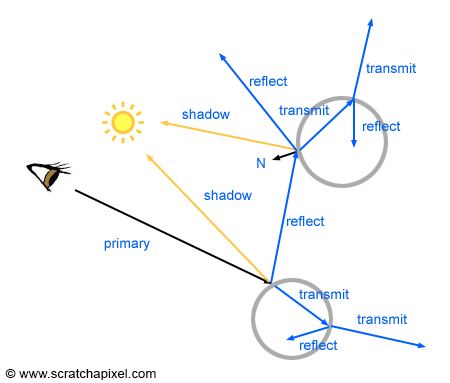
\includegraphics[width=0.8\linewidth]{rt-recursive.png}
\caption{Reflection and Refraction}
\label{fig:Reflection and Refraction}
\end{figure}
\begin{figure}[H]
\centering
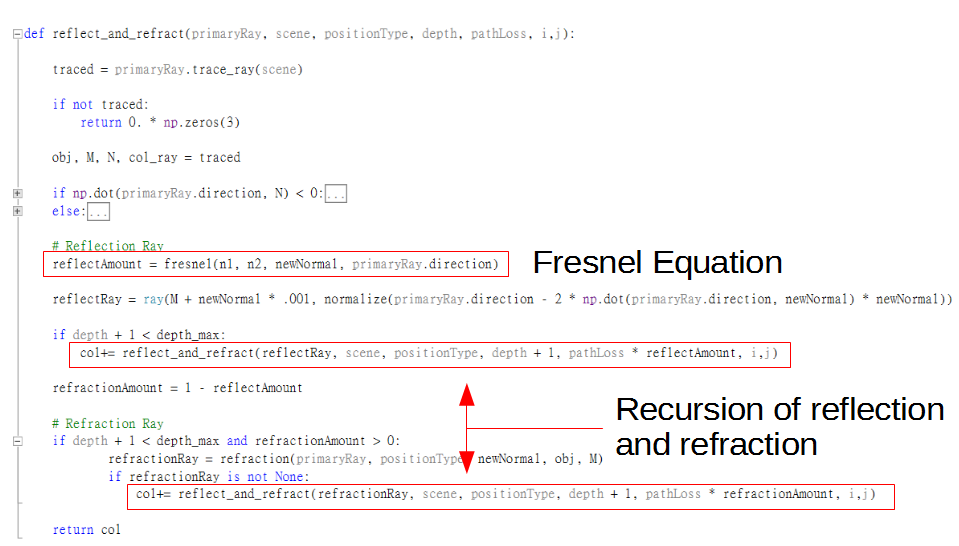
\includegraphics[width=\linewidth]{Reflect_and_refraction.png}
\caption{Recursion of reflection and refraction}
\label{fig:Recursion of reflection and refraction}
\end{figure}
\begin{figure}[H]
\centering
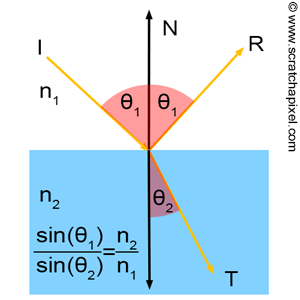
\includegraphics[scale=0.6]{shad-refraction6.png}
\caption{Fresnel Equation Parameter}
\label{fig:Fresnel Equation Parameter}
\end{figure}  

\subsubsection{Shadow Ray with Transparent Object}
In basic raytracing algorithm, when a primary ray intersects with an object, the shadow ray from the intersection point to the light will be check if it intersects another object. If it intersects with another object, that object casts a shadow and the colour of the pixel related to this primary ray is RGB(0, 0, 0) (black). However, if the object which casts a shadow is transparent, the colour should just become dimmer instead of black. Because Fresnel equation can not be used to calculate how much shadow ray transmits through an object, we use transparency level which is mentioned before to give each object a simple refractive amount. Then, we multiply the lighting of shadow ray by the simple refractive amount of objects which are intersected with it. For instance, if a shadow ray of an intersection point with colour RGB(0.5, 0.5, 0.5) intersect two object with transparency level 3 and 4, the final colour becomes RGB(0.5, 0.5, 0.5) $\times0.6\times0.8=$ RGB(0.24, 0.24, 0.24). The difference of shadow can be seen in Figure \ref{fig:Simple Refractive Amount}. The correspondence table between transparency level and the simple refractive amount we use can be seen below.

\begin{center}
    \begin{tabular}{| l | l | l}
    \hline
    Transparency Level & Simple Refractive Amount \\ \hline
    0 & 0 \\ \hline
    1 & 0.2 \\ \hline
    2 & 0.4 \\ \hline
    3 & 0.6 \\ \hline
    4 & 0.8 \\ \hline
    5 & 0.9 \\ \hline
    \end{tabular}
\end{center}

\begin{figure}[H]
\centering
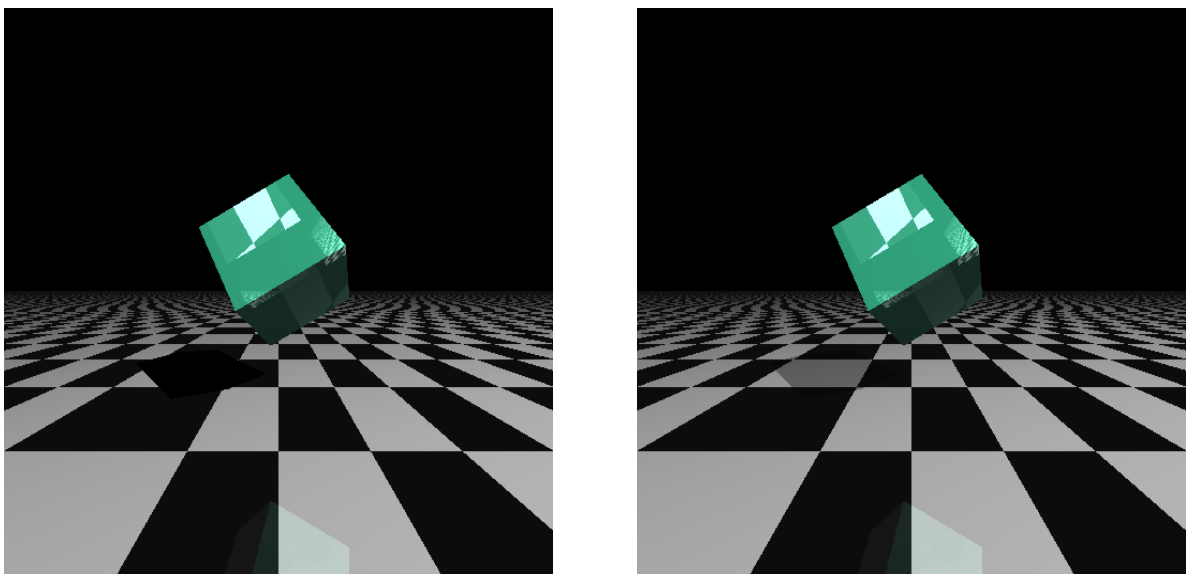
\includegraphics[scale=0.6]{Simple_Refractive_Amount.png}
\caption{Raytracing with Simple Refractive Amount (Right)}
\label{fig:Simple Refractive Amount}
\end{figure}  

\subsubsection{Camera Setting}
We use normal vector $[0, 0, 1]$ and $2\times2$ size of the raster image as a base of the camera setting. It means the direction between the camera and centre of the raster image is $[0, 0, 1]$. The software calculates the rotation angle between $[0, 0, 1]$ and input camera looking direction to generate a new normal vector of the raster image. Then, the whole process of raytracing would base on this new raster image (Figure \ref{fig:Camera Setting}). The image of different camera looking point can be seen in Figure \ref{fig:Camera_Dif}

\begin{figure}[H]
\centering
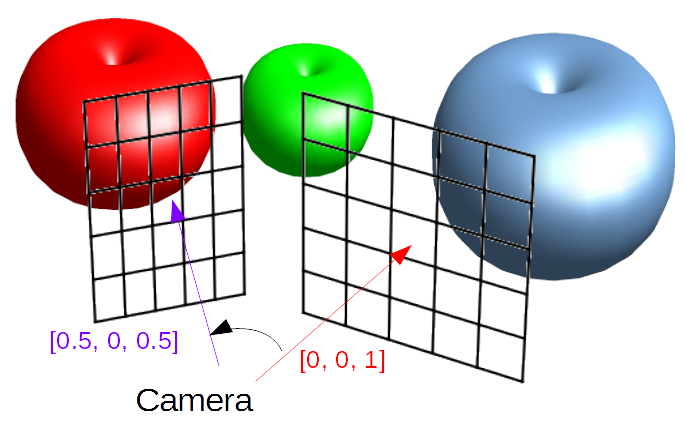
\includegraphics[width=0.6\linewidth]{Camera_Setting.png}
\caption{Camera Setting}
\label{fig:Camera Setting}
\end{figure}

\begin{figure}[H]
\centering
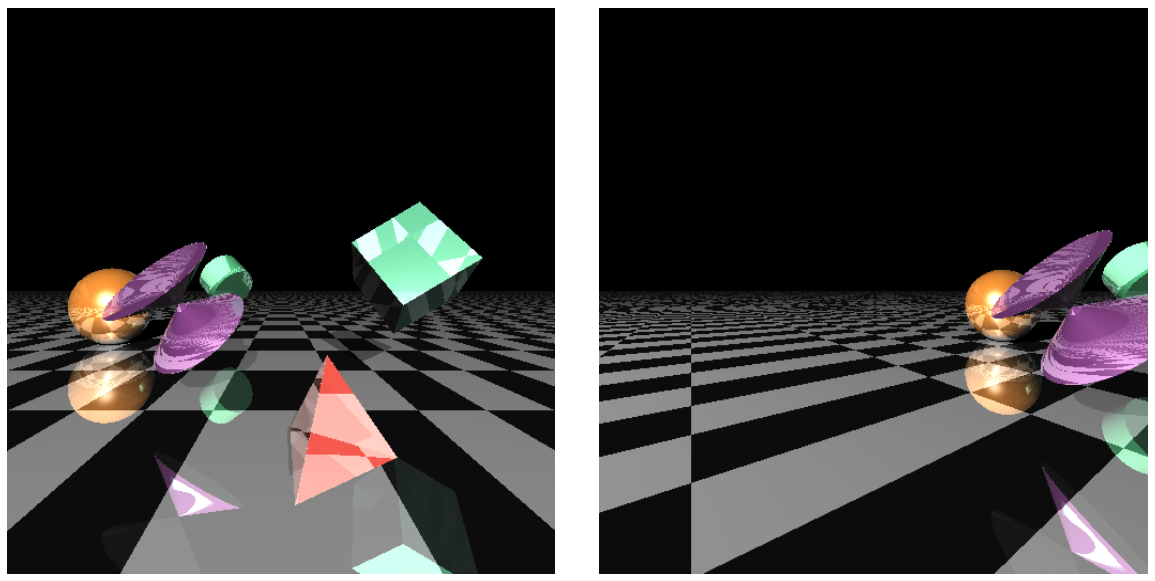
\includegraphics[width=0.6\linewidth]{Camera_Dif.png}
\caption{Different Camera Looking Point}
\label{fig:Camera_Dif}
\end{figure}

\subsubsection{Multi-processing}
Because the software has to calculate the colour of each pixel in an image, the performance is low. For example, a $512\times512$ resolution image which includes 5 objects with ray depth$=4$, there are at last  $512\times512\times5\times4$ calculations for an intersection between ray and objects. As a result, multi-processing is used to improve the performance of the software. The calculation in each pixel are independent, so we decided to divide an image into multi parts and use subprocesses to calculate for each part concurrently. In the implementation of a $512\times512$ resolution image, X-axis and Y-axis of the image are divided into 8 parts, the image is divided into 64 blocks and each block has $64\times64$ pixels. The software starts 64 subprocesses, and each subprocess generates a sub image and stores it in a queue. The main process will get all sub images from the queue and combine them to a complete image after all subprocesses finish. Theoretically, running time can be reduced to $\frac{1}{64}$ of the original version. The detail of implementation can be seen in Figure \ref{fig:Multi-Processing}.

\begin{figure}[H]
\centering
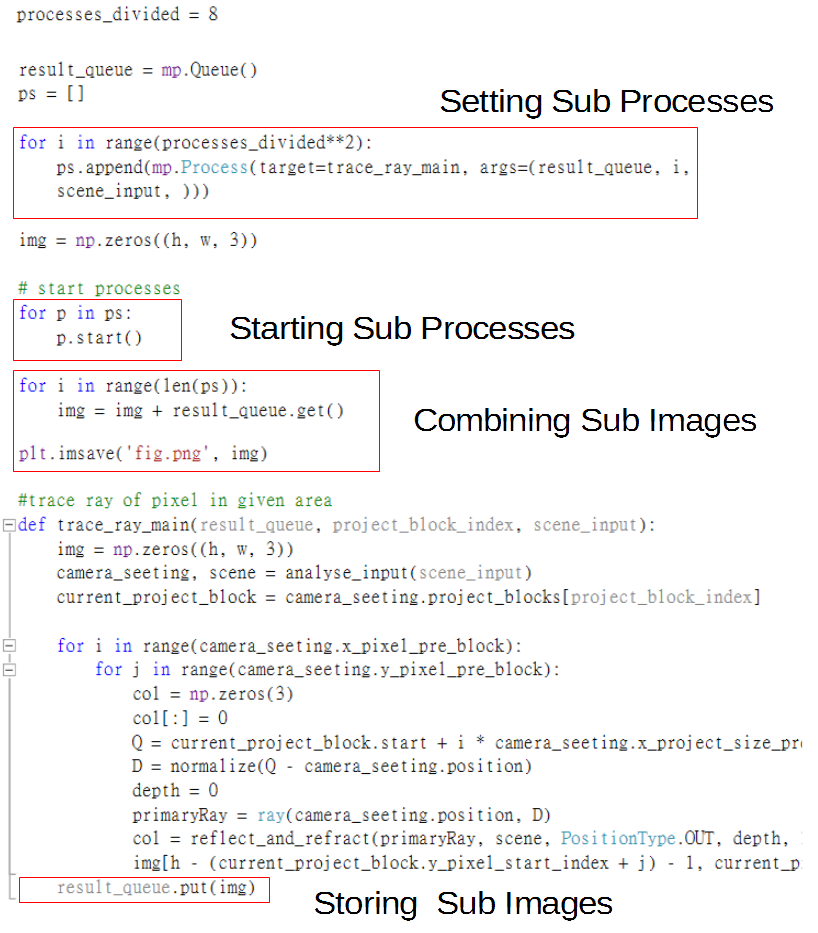
\includegraphics[width=0.8\linewidth]{Multi-processing.png}
\caption{Multi-Processing}
\label{fig:Multi-Processing}
\end{figure} 

\subsubsection{Connection Between Front-End(GUI) and Back-End(Program)}
It is necessary to design a method to connect the GUI and the back-end so that make it easier and more friendly for user to use function of program. We based on the JSON file to implement that. The whole process is as following:
\begin{enumerate}
\item Front-end offer the user GUI to set the parameters they want.
\item GUI receive the input from user (number of object, name of object, the color of object, etc.) and then generate the output file (data.json) which contain all the input data.
\item Back-end take the file (data.json) and analyze it and transmitted the parameters into program.
\item Program get the input and show the result, a good example can be shown in Figure \ref{fig:RayTracing Output}.
\end{enumerate}

\begin{figure}[H]
\centering
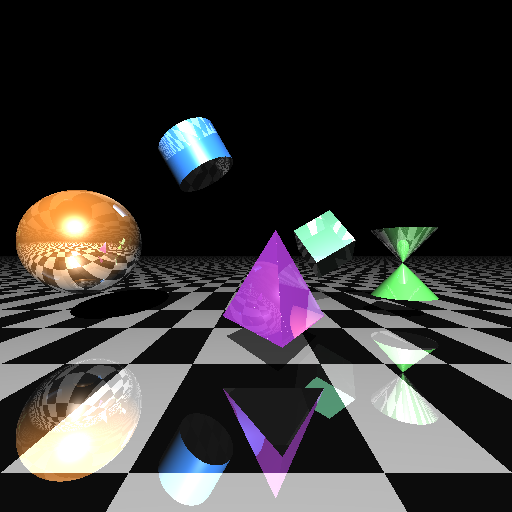
\includegraphics[width=0.8\linewidth]{Shape_all_objects.png}
\caption{RayTracing Output}
\label{fig:RayTracing Output}
\end{figure} 

The format of JSON file is shown as Figure \ref{fig:JSON File Format}

The method called 'analyse\_input' is shown as Figure \ref{fig:Analyse Input Data}

\begin{figure}[htbp]
\centering
\begin{minipage}[t]{0.38\textwidth}
\centering
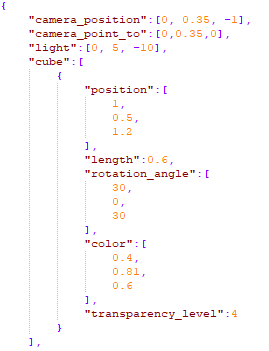
\includegraphics[width=4cm]{data_format.png}
\caption{JSON File Format}
\label{fig:JSON File Format}
\end{minipage}
\begin{minipage}[t]{0.48\textwidth}
\centering
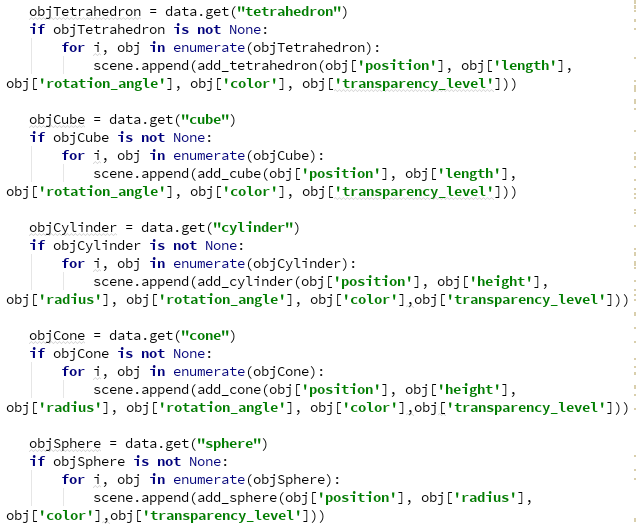
\includegraphics[width=8cm]{json_analyse.png}
\caption{Analyse Input Data}
\label{fig:Analyse Input Data}
\end{minipage}
\end{figure}

\subsubsection{Software Testing}
We did the unit testing on the smaller functions which are used in main raytracing function. For example, we tested function analyse\_input() by giving a JSON input file and checking if the output object contains all input shapes and the scene parameters are correct. Another example is function rotation() which rotates a node with a given centre point and an angle. We Know that a node [1, 0, 0] can be rotated from [0, 0, 1] with 90 degrees on Y-axis and center point [0, 0, 0], so we used these values to check if the function works correctly. We used black box testing on the main raytracing function because it is easier to find an error by observing the output image. If an unexpected image is observed, we then go through the detail of code to identify the cause and fix it. During the testing, we use around 20 test cases which have different parameters of shapes and environment to ensure the quality. 

\subsection{GUI Implementation}
Graphic user interface aims to accept user input and generate configuration file for the back-end. (The tools we used to build such user interface is Flask, which is a micro-framework for Python.) It can be separate into two parts, which are: HTML page design and Flask event response logic design. 

\subsubsection{HTML page design}
While using the user interface, users are first asked to choose how many objects to have in the scene, where we provide user with 5 options (1, 2, 3, 4 and 5). After choosing the number (for example user chose to have 2 objects), the page would be redirected to another page which accepts user input for detail information of all objects as seen in Figure \ref{fig:ObjectFeatures}.

\begin{figure}[H]
\centering
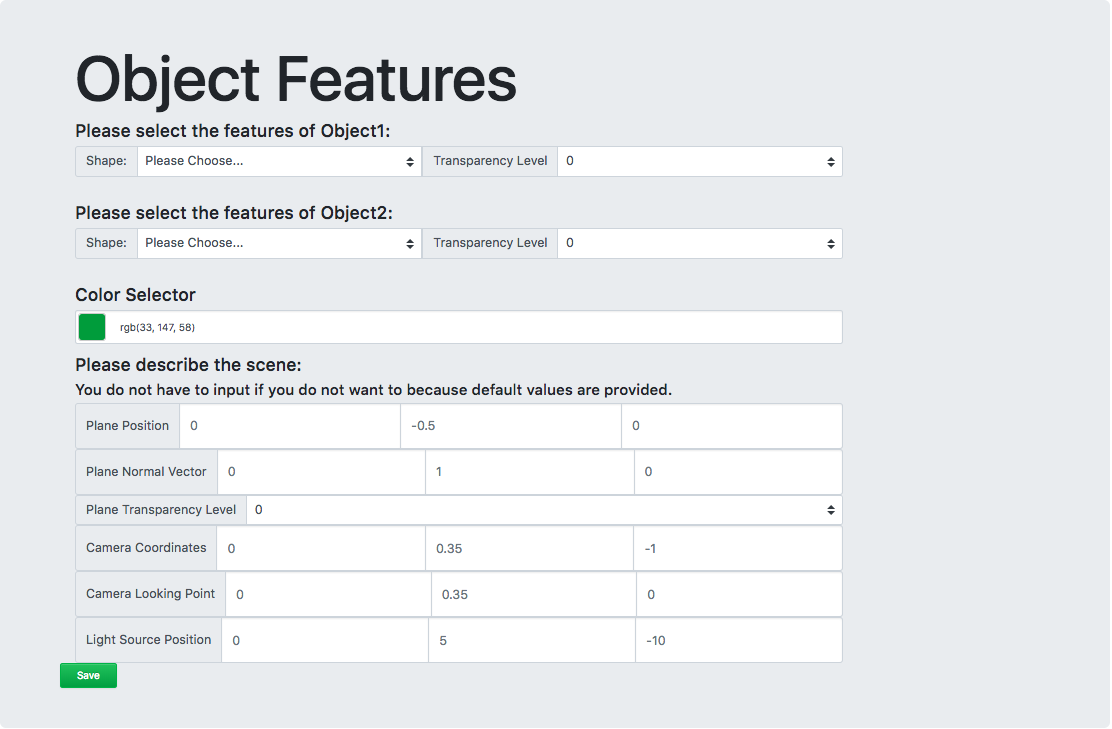
\includegraphics[width=\linewidth]{GUI_Figure1.png}
\caption{Object Features}
\label{fig:ObjectFeatures}
\end{figure}

Figure \ref{fig:ObjectFeatures} shows that users are asked to fill in all blanks to describe what the scene would look like, what are and where are all objects. Several drop-down menus are used when choosing object types and object transparency levels. For object type selection, different type of objects has different input forms as seen in Figure \ref{fig:InputForms}. And colour selector is used to support user to decide about colours. 

\begin{figure}
\centering
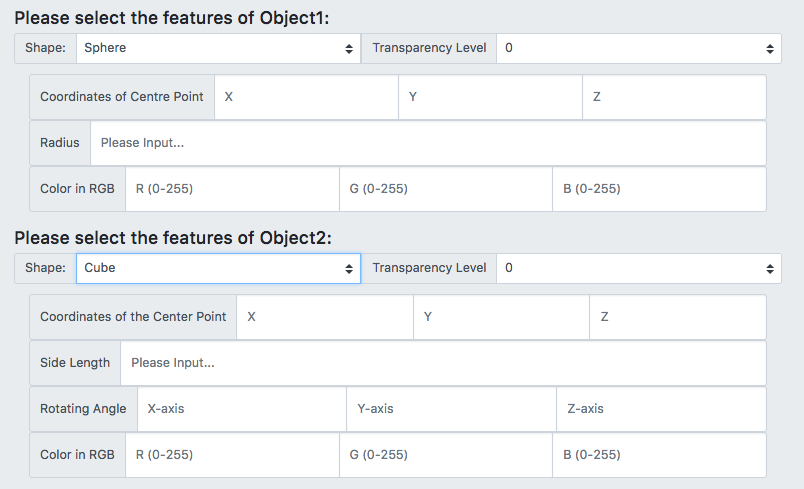
\includegraphics[scale=0.5]{GUI_Figure2.png}
\caption{Different Input Forms}
\label{fig:InputForms}
\end{figure}

After finish filling all the blanks, user can press the “Save” button which is in the bottom of the page, all the parameters would be then send to the server using Ajax, and if there is anything wrong about user input, there will be an alert message.

\subsubsection{Flask Event Response Logic Design}
Event response in GUI is using HTML post/request method and Ajax. Alert message would come out if some blanks are missing while user trying to set objects or characters are written in any blank.

After receiving JSON format data posted from the HTML file by Ajax which includes parameters of objects and the scene, the back-end need to pack these data into appropriate format for ray-tracing program.  To do this, we added a new class called “OutputGenerator”, which generates the right data format for each type of object and add it in the list of corresponding object type. When a user is done with parameter setting, the JSON file which connects the graphic user interface to the ray tracing program can be generated by calling Generate\_File() function in this class as seen in Figure \ref{fig:OutputGenerator}.

\begin{figure}[htb]
\centering
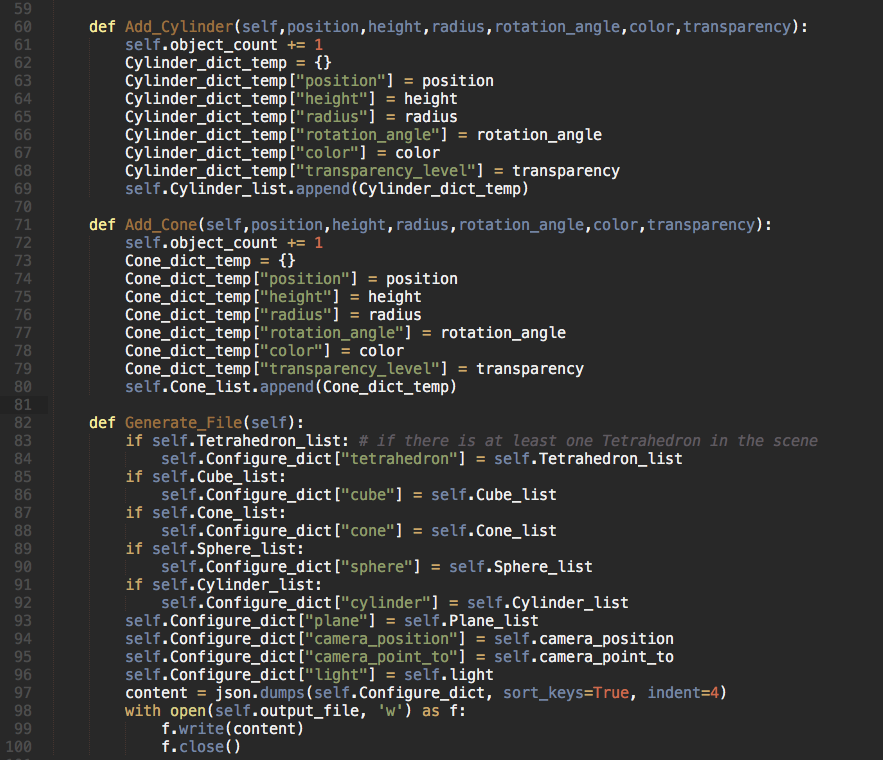
\includegraphics[width=12cm]{GUI_Figure3.png}
\caption{Class OutputGenerator}
\label{fig:OutputGenerator}
\end{figure}

\subsubsection{Software Testing}
Graphic user interface is implemented by flask web-based framework, users can access to the system by laptops, desktops, or by smart phones. However, it did not support multi-user working at the same time because that would add more objects to the ending of the JSON file which used to describe objects and the scene. When a user leaves a blank or inputs some characters in forms, an alert message would come out as seen in Figure \ref{fig:GUI_Figure4}.

\begin{figure}[h!]
  \centering
  \begin{subfigure}[b]{1\linewidth}
    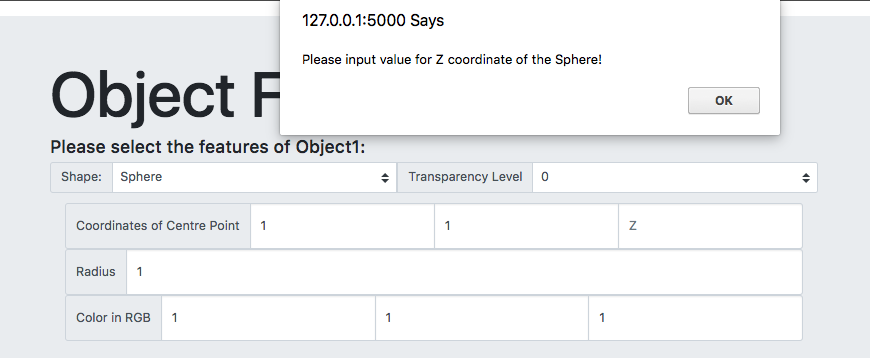
\includegraphics[width=\linewidth]{GUI_Figure4a.png}
    \caption{No Blanks Allowed}
  \end{subfigure}
  \begin{subfigure}[b]{1\linewidth}
    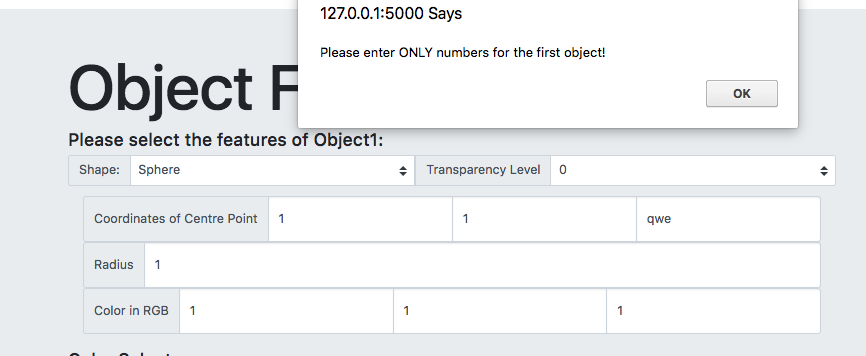
\includegraphics[width=\linewidth]{GUI_Figure4b.png}
    \caption{Only Digits Allowed}
  \end{subfigure}
  \caption{Rejected Erroneous Inputs}
  \label{fig:GUI_Figure4}
\end{figure}

All the colour input should be only including number between 0 and 255, with at most one dot, and dot could not be in the beginning of the number. If user miss input something, there will be an alert message as seen in Figure \ref{fig:GUI_Figure5}.


\begin{figure}[!htb]
\centering
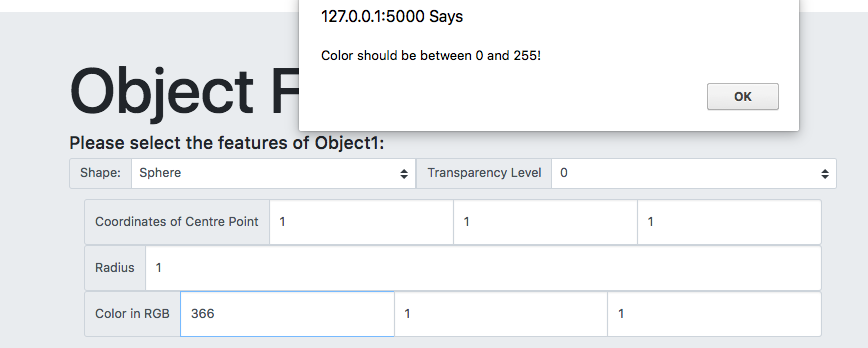
\includegraphics[scale=0.5]{GUI_Figure5.png}
\caption{Incorrect Colour Input}
\label{fig:GUI_Figure5}
\end{figure}

%% Team Work
\section{Team Work}

The team was initially divided into groups of two, each having a specific task in the project. The first group handled the Shapes Design and Implementation, assigned to Mohammad Omdah \& Shiyu Zhang. The second group handled the RayTracing Integration and Implementation, assigned to Xiang Li \& Nien-Tsu Cou. Finally, the third group handled the GUI Interface, assigned to Ahmad Alkhoory \& Zihao Zhao.

The three sub groups had a wonderful collaboration and efficient communication between them, and assuring that was our first objective before starting with the technicality of the project. As the group had it's first meeting, certain communication tools have been identified, weekly meetings have been assigned, and task's division have been agreed upon.

Communication tools were carefully selected between the vast choices available in hand, the selected tools had to be efficient, multi-platform product, and easy to use. Whatsapp was the group's number one application, mainly used as a platform for tasks discussions, meetings updates, and urgent deadlines. Overleaf was our LaTex interpreter in documenting the Initial and the Final report. Overleaf featured a real-time preview of our LaTex codes, real-time collaboration with our colleagues, as well an efficient way for identifying syntax errors. Finally, GitHub repository was used for our code development, which greatly benefited the team in tracking each group's progress.

Weekly meetings were assigned to take place every Friday, at 10 am through Skype. Those meetings were very beneficial to the whole group, where it was the time in the week were every individual showed what he have achieved, what he is currently working on, and what he is going to do next. This gave a kind of inspiration to the active groups, as well as a motivation to the slow ones.

%% Evaluation
\section{Evaluation}
This section evaluates the project from two aspects which are project progress and software. The former evaluates the way that we achieved our plan, and the latter describes the strength and weakness of the software. Finally, it will show some future work which can be done to improve the software weakness. 

\subsection{Project Progress}
The early start and regular progress are key to achieve the project for us. Because the work division was done in the early stage of the project, each member can focus on their task at the same time. Also, the progress of each member is checked every week; we finished the basic requirement of software two weeks before the deadline. Therefore, we have sufficient time for the report and thinking about improving the software.

Communication plays an important role in sharing the experience and speeds up the progress. At first, all members do not have any experience related to ray tracing. Therefore, we decided to give everyone a week to study this topic; then we have a meeting to discuss and share each one’s understanding. This help everyone to understand the topic more quickly because it cost less time to understand if someone explain to you. Also, it reduced the time of double work. In addition, members shared some useful information such as raytracing or latex tutorial website. Because of frequent communication, the status of progress is known by all group member; then the problem can be found and solved as soon as possible.

However, ray tracing is an unfamiliar topic to our group, so we did not have a big picture of what software should look like and didn’t write any specification of our software before implementation. As a result, sometimes we did the design and implementation at the same time, the work of sub groups cannot be matched currently at first such as the link between GUI and ray tracing back end. Then we had to spend more time to communicate and do the testing together.

\subsection{Strength and Weakness}
The GUI of the software is developed on a web-based platform, so it easy to use for any device which has a browser. Users do not have to use specific operating system or install any specific software on their device. However, the User describes the scene by completing the form in GUI, and it may be not easy to link the description to the what picture looks like. Therefore, shapes may be put in a position where camera covers. If the user is not satisfied with the image, they have to reset the input.

Also, performance is another issue. Because the performance of python is worse than other program languages such as C or JAVA, even we use multi-processing to reduce the running time, it still takes almost one minute to generate the image.

\subsection{Degree of Completion}
\begin{enumerate}
\item Complete

In the end of the project, we finished almost all part that mentioned in the initial report. Besides, more new ideas were came up with and we made them come true. The following is outline:
\begin{itemize}
\item Rational division of responsibility
\item Integrated Front-End(GUI)
\item Integrated Back-End(Program)
\item Diversified shapes: Sphere, Cube, tetrahedron, cylinder and cone
\item Enhanced performance: the running speed is faster than the old version by using multiprocessing.
\item Web-based support: In the initial plan, we only support the program run locally. Now we put the software on the cloud server so that everyone who has the Internet connection can run the software remotely.
\end{itemize}
\item Incomplete

Due to the time limitation, we made some changes on initial plan or skip some unimportant functions.
\begin{itemize}
\item Didn't add 'Hat' object as the shape.
\item Didn't apply the multiple platform support(only windows version), but we think the cloud server make up that shortness.
\end{itemize}
\end{enumerate}


\subsection{Future Work}
There are some functionalities of the software which we can improve. The software only allows the user to choose five types of shape; all shapes are very simple such as sphere, cube. Although we considered combining with multi simple shapes to a complicated shape, it would take more time to generate the image. If we can improve the performance issue in the future, the variety of shapes can also increase. Also, we can use a dynamic setting of diffuse and specular for each subject instead of using a default value. It can perform difference of material and make an image more realistic. 

To improve the description of a scene in GUI, We can add the three view diagram to allow users to preview the result. Users can easily know the relative position of objects and the chance of that the image is not satisfied by the user such as objects overlapping.  

%% Peer Assessment
\section{Peer Assessment}
There are 5 criteria the team has agreed to do peer assessment:
\begin{itemize}
\item Deadline: commit in the task deadline which assigned to each member, the points for deadline is 20.
\item Performance: performance of each member to achieve his tasks with deadline with expected results,the points for performance is 20. 
\item Tasks Reporting: each group member report the issues, tasks, help if needed and requests, so for each of them 5 points and the total for task reporting 20 points.
\item Meeting Attendance:   the team did 15 meetings in this 11 weeks term each will weighted 1.3, the points for meeting attendance is 20.
\item Contributions: This include contribution on github, reporting final presentation and report, help other team members and code, so for each of them 5 points and the total for contribution 20 points. Below Figure \ref{fig:Peerass} is the agreed results of team assessment:

\begin{figure}[ht]
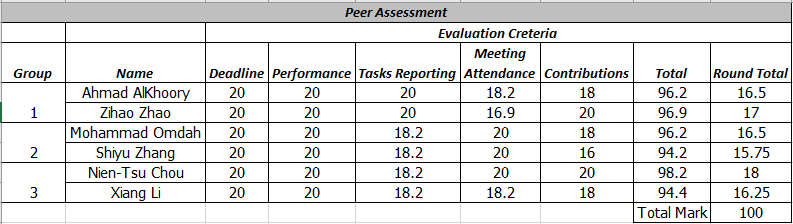
\includegraphics[width=\linewidth]{peer_assessment.PNG}
\caption{Peer Assessment Criteria}
\label{fig:Peerass}
\end{figure}

\end{itemize}

%% Review
\section{Review}
This website (https://app.pluralsight.com) was helpful to understand python fundamental. It is not free courses, but recommended from many expert in technology fields. The cost had been paid to understand python programming language.
\subsection{Shapes Design Review}
Below are websites have been helped to understand the ray tracing, python code and how to use latex:

This website(https://www.sharelatex.com/learn) was helpful to understand how to write equations, add images, tables, sections, subsection and formatting for latex document.

This website (https://www.khanacademy.org/partner-content/pixar/rendering/rendering1/v/renderin) was helpful to understand ray tracing function as beginner and create your own image from calculation.

\subsection{Raytracing Review}
Learn Computer Graphics From Scratch \cite{Learn Computer Graphics From Scratch} is the main  source for us to understand the basic knowledge and implementation of ray-tracing. It includes mathematics of interaction between ray and shape, shadow, reflection and refraction. These information help us to achieve our requirement and design. In addition, our back-end ray-tracing program is based on Very simple ray-tracing engine in (almost) pure Python \cite{Very simple ray-tracing engine in (almost) pure Python}. 

\subsection{GUI Review}
Bootstrap (http://getbootstrap.com) was the main tool for our GUI program. From Bootstrap, we used all of our buttons, drop down selection, forms, as well as our fonts and containers. Bootstrap greatly enhanced our GUI graphics to be user friendly, as well as portable to multi platform web browsers.


\begin{thebibliography}{9}

\bibitem{Ray tracing}
What is ray tracing? Everything you need to know about the next big graphical leap. [online] Available at: https://www.techradar.com/news/ray-tracing [Accessed 21 Mar. 2018]

\bibitem{kivy} 
Kivy. [online] Available at: https://kivy.org/home [Accessed 15 Mar 2018].

\bibitem{Ray tracing primitives} 
Dodgson, N. and Blackwell, A. (1999). Ray tracing primitives. [online] Available at: https://www.cl.cam.ac.uk/teaching/1999/AGraphHCI/SMAG/node2.html [Accessed 21 Mar. 2018].

\bibitem{Learn Computer Graphics From Scratch}
Learn Computer Graphics From Scratch. [online] Available at: https://www.scratchapixel.com [Accessed 21 Mar. 2018].

\bibitem{Very simple ray-tracing engine in (almost) pure Python}
Rossant, C. (2017). Very simple ray tracing engine in (almost) pure Python. [online] Available at: https://gist.github.com/rossant/6046463 [Accessed 01 Feb. 2018].
\end{thebibliography}


\end{document}

